\section{Part II: Auto-configuration}

\begin{frame}{Why ML-based NIDS still need explicit adaptation}
	\small

	\begin{columns}[T,onlytextwidth]
		\column{0.40\linewidth}
		\begin{itemize}
			\item ML-based NIDS are trained on historical traffic and deployed as static detectors.
			\item This assumes training and deployment traffic remain statistically close.
			\item In practice, benign traffic evolves, and attackers adapt.
		\end{itemize}

		\column{0.58\linewidth}
		\centering

		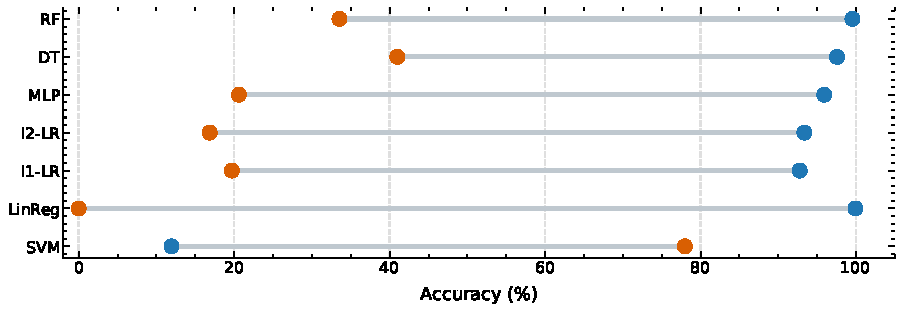
\includegraphics[width=\linewidth,height=0.32\textheight,keepaspectratio]{figures/auto_configuration/kdd_distribution_shift.pdf}

		\par\vspace{0.05em}
		{\fontsize{5.2}{6}\selectfont \textcolor{blue}{\textbf{Blue:}} Shifted benign traffic \quad \textcolor{orange}{\textbf{Orange:}} Shifted malicious traffic\par}

		\par\vspace{0.1em}
		\figsource{Anderson \& McGrew, KDD 2017, Table 2}

		\vspace{0.3em}

		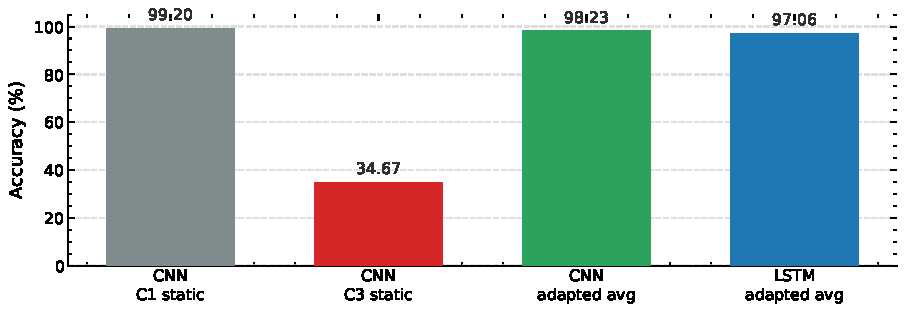
\includegraphics[width=\linewidth,height=0.32\textheight,keepaspectratio]{figures/auto_configuration/qiao_concept_drift.pdf}

		\par\vspace{0.1em}
		\figsource{Qiao et al., IEEE TII 2022, Table V/VI and Section IV-C}
	\end{columns}

	\vspace{0.15em}
	\centering
	\resizebox{\linewidth}{!}{\textbf{$\Rightarrow$ Detection performance can degrade after deployment $\Rightarrow$ explicit adaptation mechanisms are needed}}
\end{frame}

\definecolor{famdrift}{HTML}{3B82F6}
\definecolor{famonline}{HTML}{0F766E}
\definecolor{famactive}{HTML}{D97706}
\definecolor{famtransfer}{HTML}{7C3AED}
\definecolor{fammeta}{HTML}{C026D3}
\definecolor{famthresh}{HTML}{6B7280}

\newcommand{\familymarker}[1]{\tikz[baseline=-0.55ex]\fill[#1] (0,0) circle (0.9ex);}
\newcommand{\familyname}[2]{\familymarker{#1}\hspace{0.35em}\textbf{#2}}
\newcommand{\adaptfamilyrow}[7]{%
	\uncover<#1->{\familyname{#2}{#3}} &
	\uncover<#1->{\tiny #4} &
	\uncover<#1->{#5} &
	\uncover<#1->{#6} &
	\uncover<#1->{#7} \\
	\addlinespace[0.12em]}

\begin{frame}{State of the art: main adaptation families}
	\fontsize{6.15}{6.85}\selectfont
	\renewcommand{\arraystretch}{1.04}
	\setlength{\tabcolsep}{4pt}

	\begin{tabular}{
		>{\raggedright\arraybackslash}p{2.0cm}
		>{\raggedright\arraybackslash}p{2.25cm}
		>{\raggedright\arraybackslash}p{2.75cm}
		>{\raggedright\arraybackslash}p{3.2cm}
		>{\raggedright\arraybackslash}p{1.55cm}}
		\toprule
		\textbf{Family} & \textbf{Representative methods} & \textbf{Operational need} & \textbf{Adaptation mechanism} & \textbf{Label budget} \\
		\midrule
		\adaptfamilyrow{2}{famdrift}{Drift detection}{CADE, OWAD, TRANSCEND}{Early warning of drift}{Shift monitoring in data or outputs}{None}
		\adaptfamilyrow{3}{famonline}{Online / continual learning}{AOC-IDS, ENIDrift, ReCDA}{Long-term tracking of evolving traffic}{Incremental weight updates from traffic streams}{Zero to low}
		\adaptfamilyrow{4}{famactive}{Active / semi-supervised}{Active-SVDD, HITL-IDS, METALS}{Adaptation under scarce labels}{Label queries and pseudo-label exploitation}{Minimal}
		\adaptfamilyrow{5}{famtransfer}{Transfer / domain adaptation}{ADA, NAEF, DI-NIDS}{Deployment to a new network context}{Knowledge transfer across domains}{Zero to few}
		\adaptfamilyrow{6}{fammeta}{Meta-learning}{FC-Net, PTN-IDS, RETSINA}{Fast adaptation with limited data}{Learned initialization or metric}{Few to zero}
		\adaptfamilyrow{7}{famthresh}{Threshold / score calibration}{Bridges, Hundman, MAGPIE}{Alert control without retraining}{Threshold or score adjustment}{None to very low}
		\bottomrule
	\end{tabular}

	\vspace{0.18em}
	\only<8>{%
		\begin{beamercolorbox}[wd=\linewidth,sep=0.45ex,rounded=true]{block body}
			\scriptsize
			\begin{columns}[T,onlytextwidth]
				\column{0.29\linewidth}
				\familymarker{famdrift}\ \textbf{Change monitoring only}\\[-0.02em]
				{\tiny No direct detector adaptation.}

				\column{0.39\linewidth}
				\familymarker{famonline}\hspace{0.08em}\familymarker{famactive}\hspace{0.08em}\familymarker{famtransfer}\hspace{0.08em}\familymarker{fammeta}\ \textbf{Model-targeted adaptation}\\[-0.02em]
				{\tiny Weights, transferred repr., learned init.}

				\column{0.30\linewidth}
				\familymarker{famthresh}\ \textbf{Threshold / HP adaptation}\\[-0.02em]
				{\tiny Post-training HP only; not model adaptation.}
			\end{columns}
		\end{beamercolorbox}}

	\only<9>{%
		\centering
		\small\textbf{$\Rightarrow$ Existing methods mainly adapt the model or its outputs, while train-time hyperparameters remain largely fixed.}}
\end{frame}

\begin{frame}{Is hyperparameter configuration important?}
	\small

	\begin{columns}[T,onlytextwidth]
		\column{0.38\linewidth}
		\begin{itemize}
			\footnotesize
			\setlength\itemsep{0.35em}
			\item Bilot et al. re-evaluate eight state-of-the-art PIDSs in a unified framework.
			\item Tuned and untuned variants are compared under the same task.
			\item Large performance gaps reveal strong hyperparameter sensitivity.
			\item Tuning therefore affects both detection performance and the fairness of empirical comparisons.
		\end{itemize}

		\column{0.60\linewidth}
		\centering
		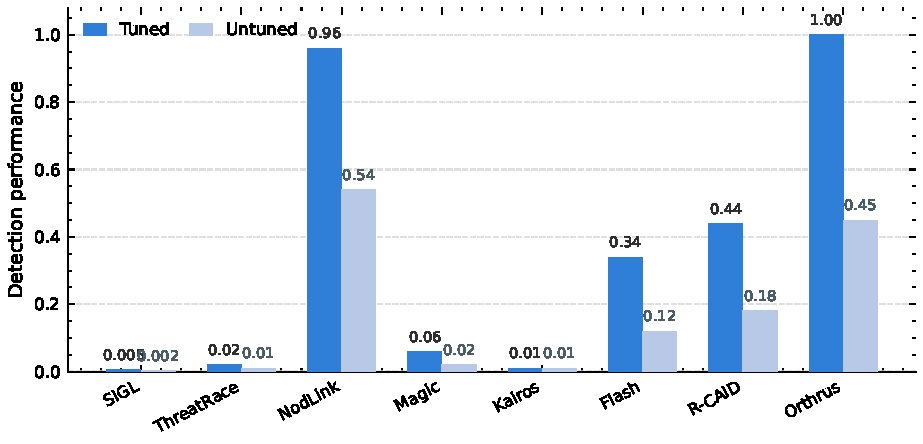
\includegraphics[width=\linewidth]{figures/auto_configuration/bilot_hpo_importance.pdf}

		\par\vspace{0.1em}
		\figsource{Bilot et al., USENIX Security 2025, Figure 5}
	\end{columns}

	\vspace{0.2em}
	\centering
	\footnotesize\textbf{$\Rightarrow$ A deeper analysis of hyperparameter impact is provided in our paper}\\[-0.05em]
	\footnotesize\textbf{\emph{An Empirical Study on Configuration Robustness of Unsupervised IDS}, accepted to the IEEE/IFIP NOMS 2026 main track.}
\end{frame}

\begin{frame}{How is configuration handled today?}
	\small

	\begin{block}{Conventional offline HPO}
		\begin{itemize}
			\setlength\itemsep{0.45em}
			\item Grid search, random search, Bayesian optimization, and evolutionary search.
			\item Repeated train-and-validate evaluations over candidate configurations.
		\end{itemize}
	\end{block}

	\vspace{0.35em}
	\begin{block}{Why not for ML-based NIDS adaptation?}
		\footnotesize
		These methods are static, offline, computationally expensive, and time-consuming procedures
		that must be re-run from scratch when the network context changes.
	\end{block}

	\vspace{0.25em}
	\begin{block}{A NIDS-specific example}
		\footnotesize
		In Anser et al. (NOMS 2023), Bayesian optimization of a binary Random Forest NIDS used
		\textbf{300 iterations} for a single daily network context, which corresponds to about
		\textbf{50 minutes} when one HPO iteration takes up to \textbf{10 seconds}.
	\end{block}

	\vspace{0.18em}
	\centering
	{\fontsize{5.8}{6.5}\selectfont Refs: Bergstra \& Bengio, JMLR 2012; Snoek et al., NeurIPS 2012; Anser et al., NOMS 2023.}
\end{frame}

\begin{frame}{Research question (RQ1)}
	\small

	\begin{block}{Research question}
		How can we find a configuration of a ML-based NIDS in a timely manner while maintaining an acceptable level of detection performance, considering a heterogeneous network context?
	\end{block}

	\vspace{0.35em}
	\begin{block}{From our analysis of hyperparameter impact}
		\begin{itemize}
			\item A NIDS configuration method has to be applied at each network context change.
			\item A new network context is defined by a new attack in the network or by a topology change.
		\end{itemize}
	\end{block}

	\vspace{0.2em}
	\centering
	\small\textbf{$\Rightarrow$ Auto-configuration via meta-learning}
\end{frame}

\begin{frame}{Auto-configuration via Meta-learning}
	\centering
	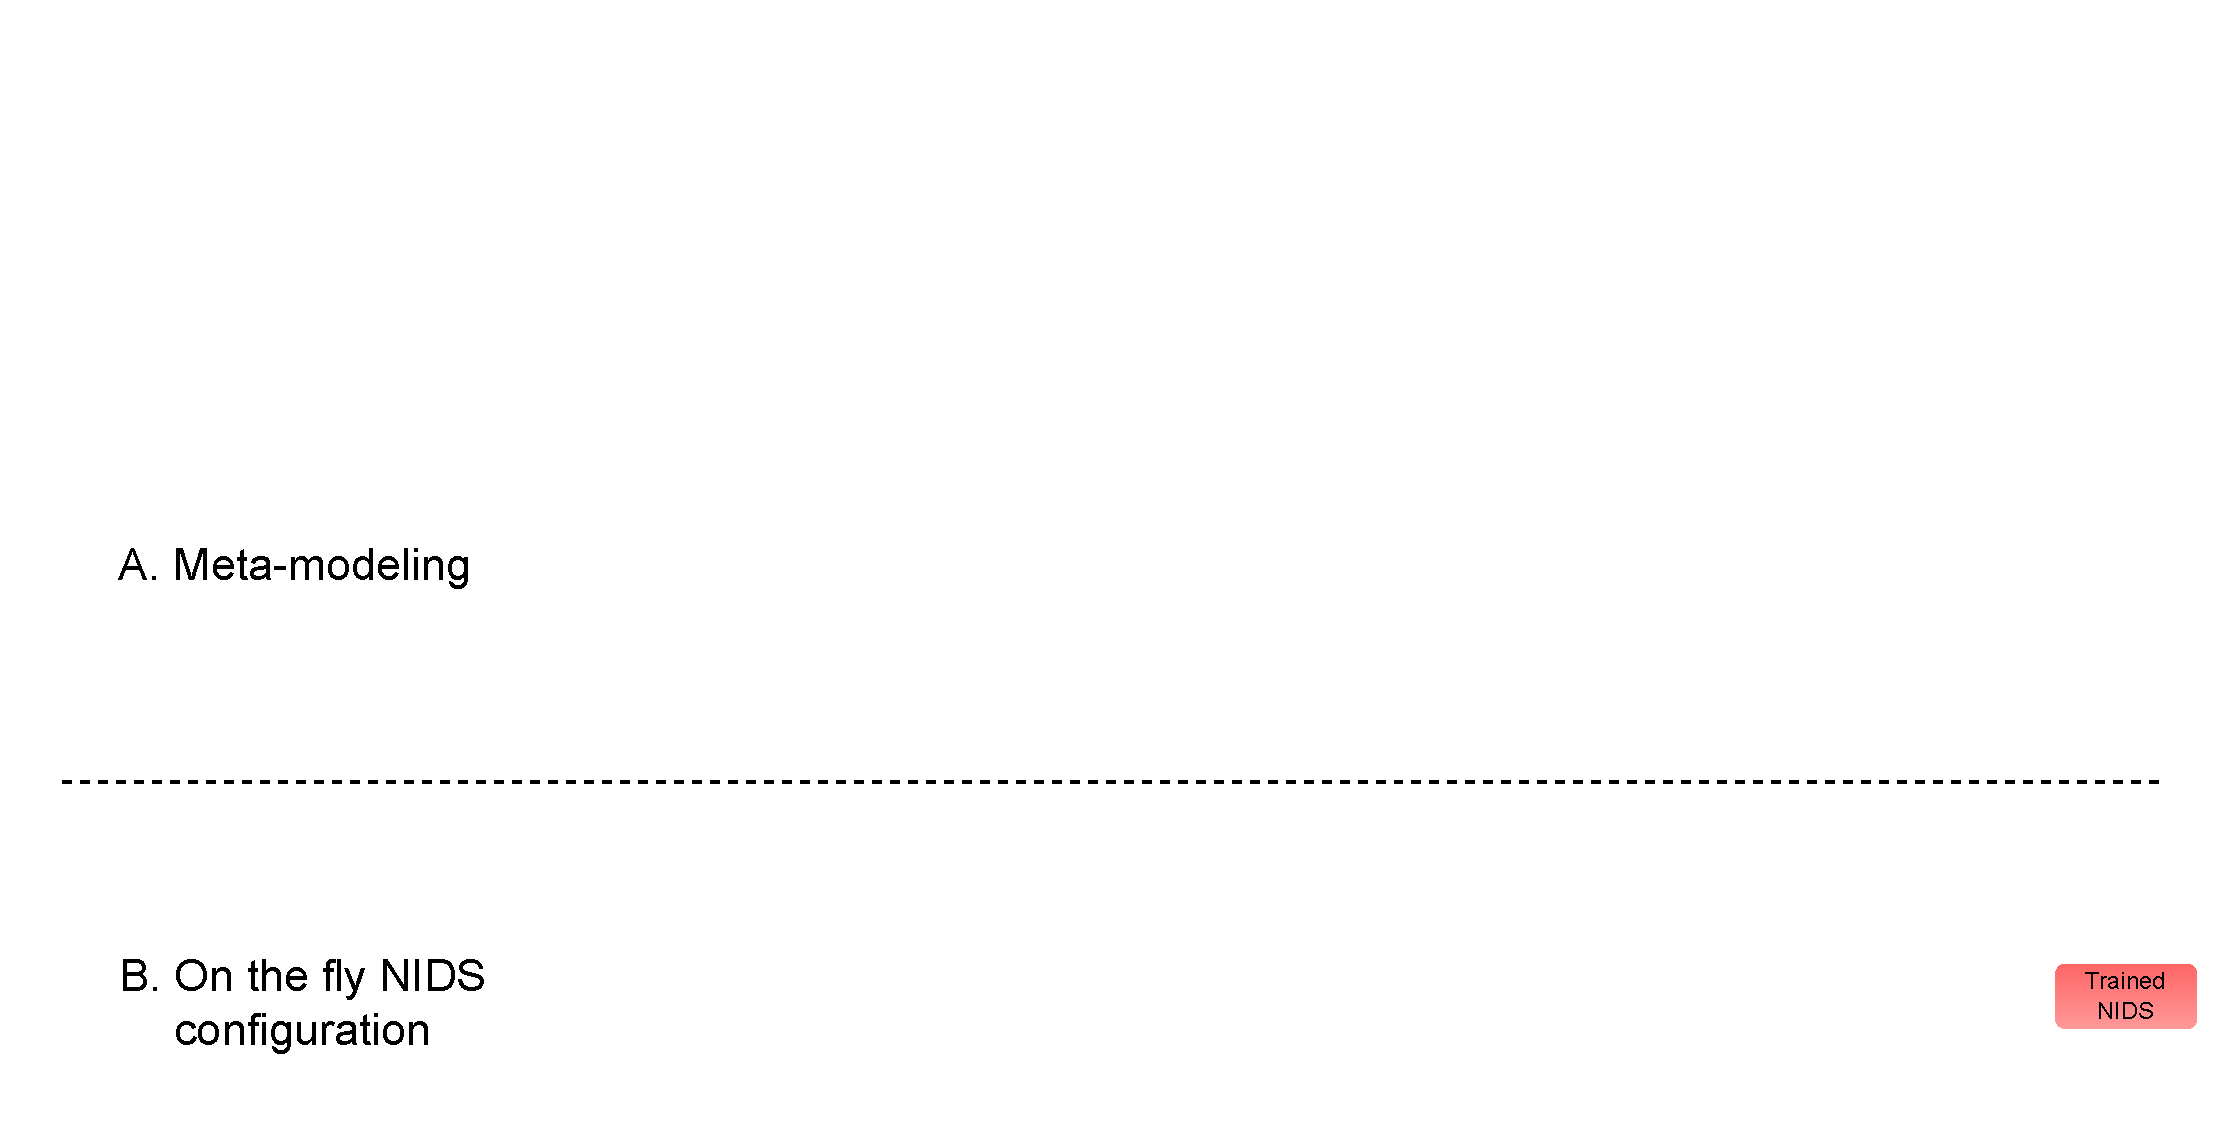
\includegraphics[width=\linewidth]{figures/auto_configuration/method/secondPartPage1.pdf}
\end{frame}

\begin{frame}[noframenumbering]{Auto-configuration via Meta-learning}
	\centering
	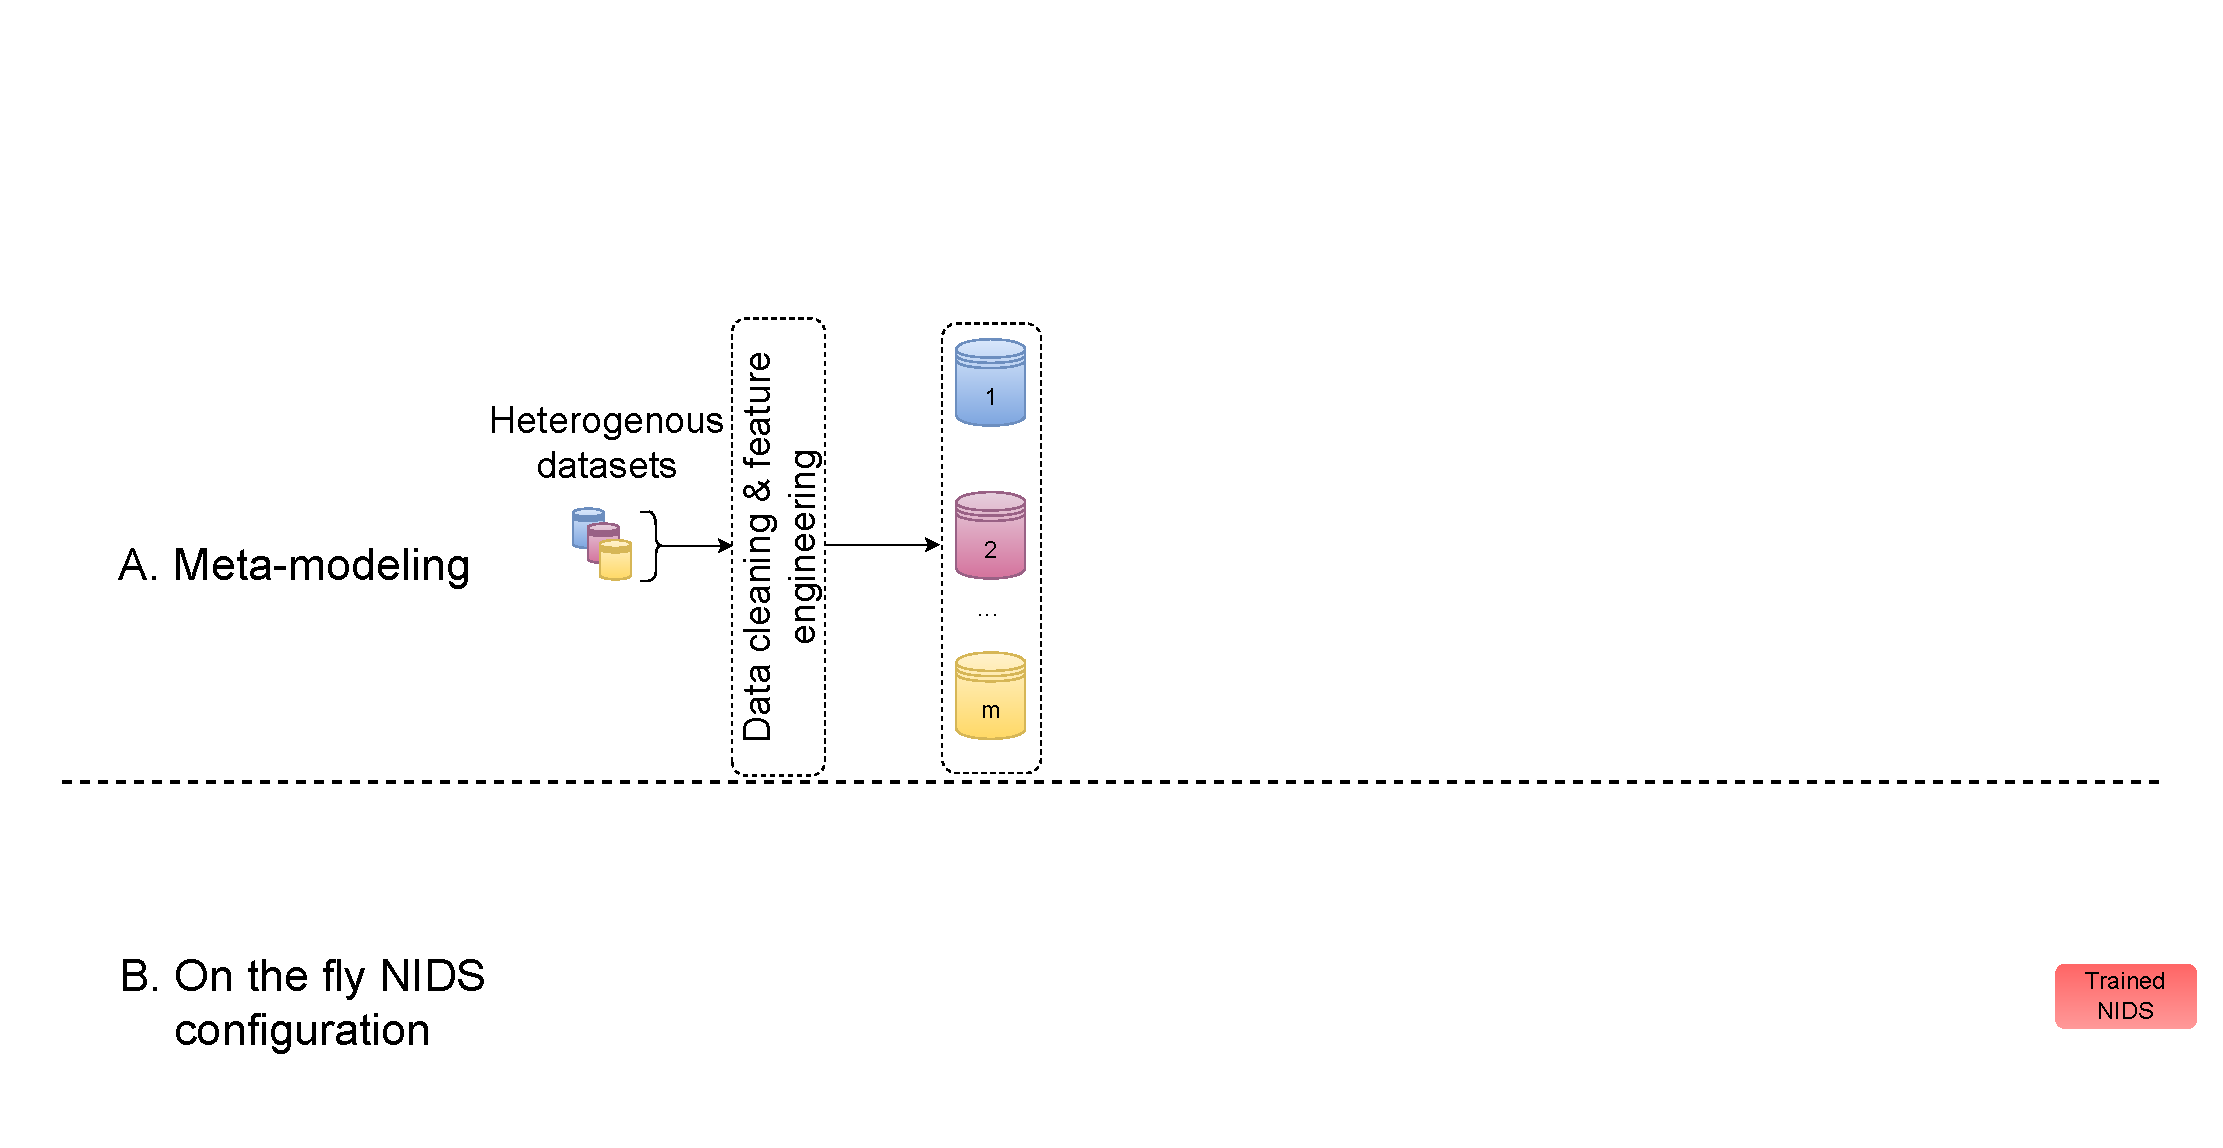
\includegraphics[width=\linewidth]{figures/auto_configuration/method/secondPartPage4.pdf}
\end{frame}

\begin{frame}[noframenumbering]{Auto-configuration via Meta-learning}
	\centering
	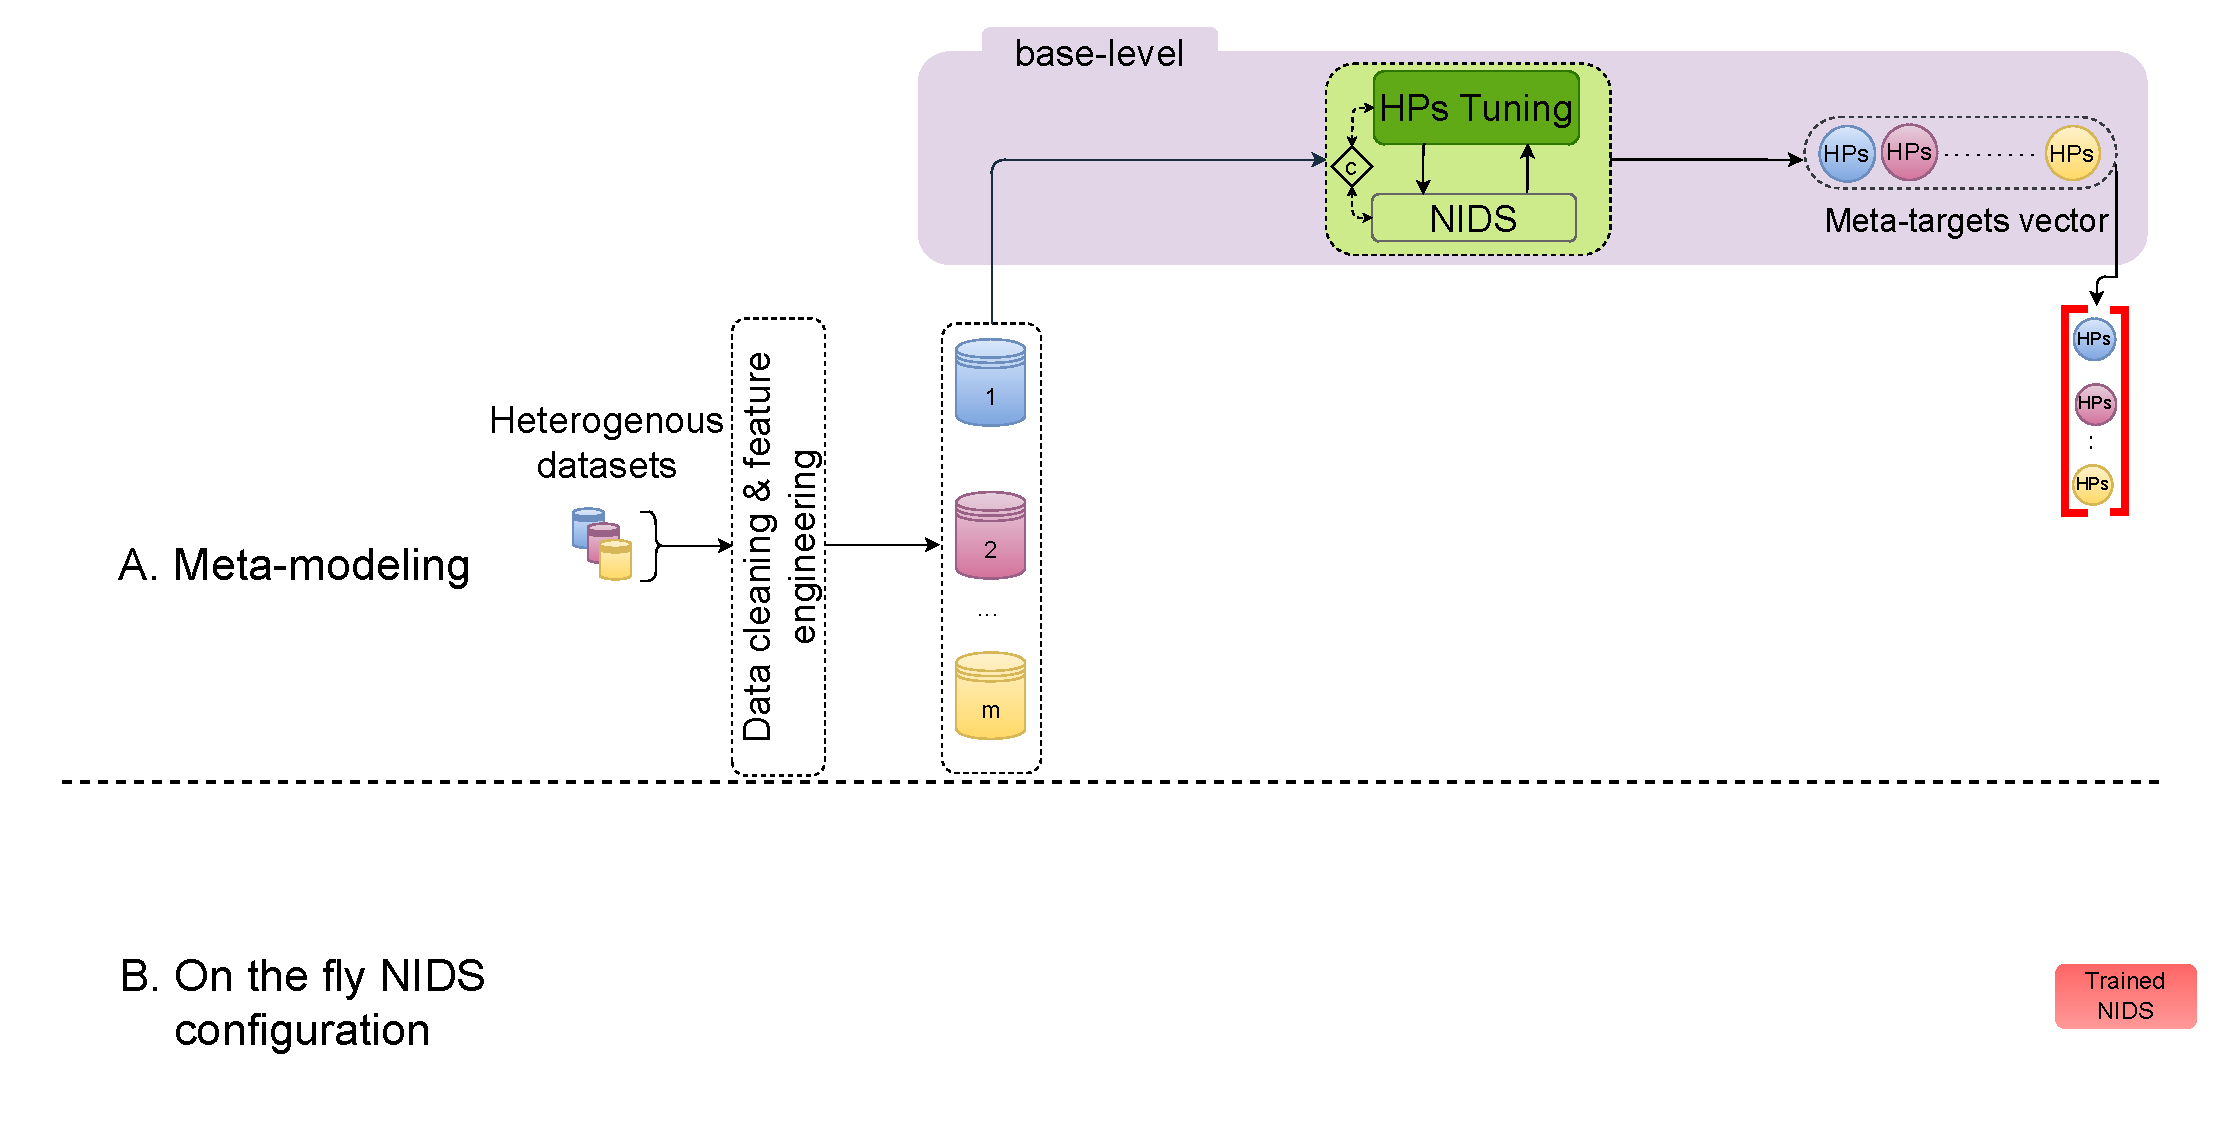
\includegraphics[width=\linewidth]{figures/auto_configuration/method/secondPartPage5.pdf}
\end{frame}

\begin{frame}[noframenumbering]{Auto-configuration via Meta-learning}
	\centering
	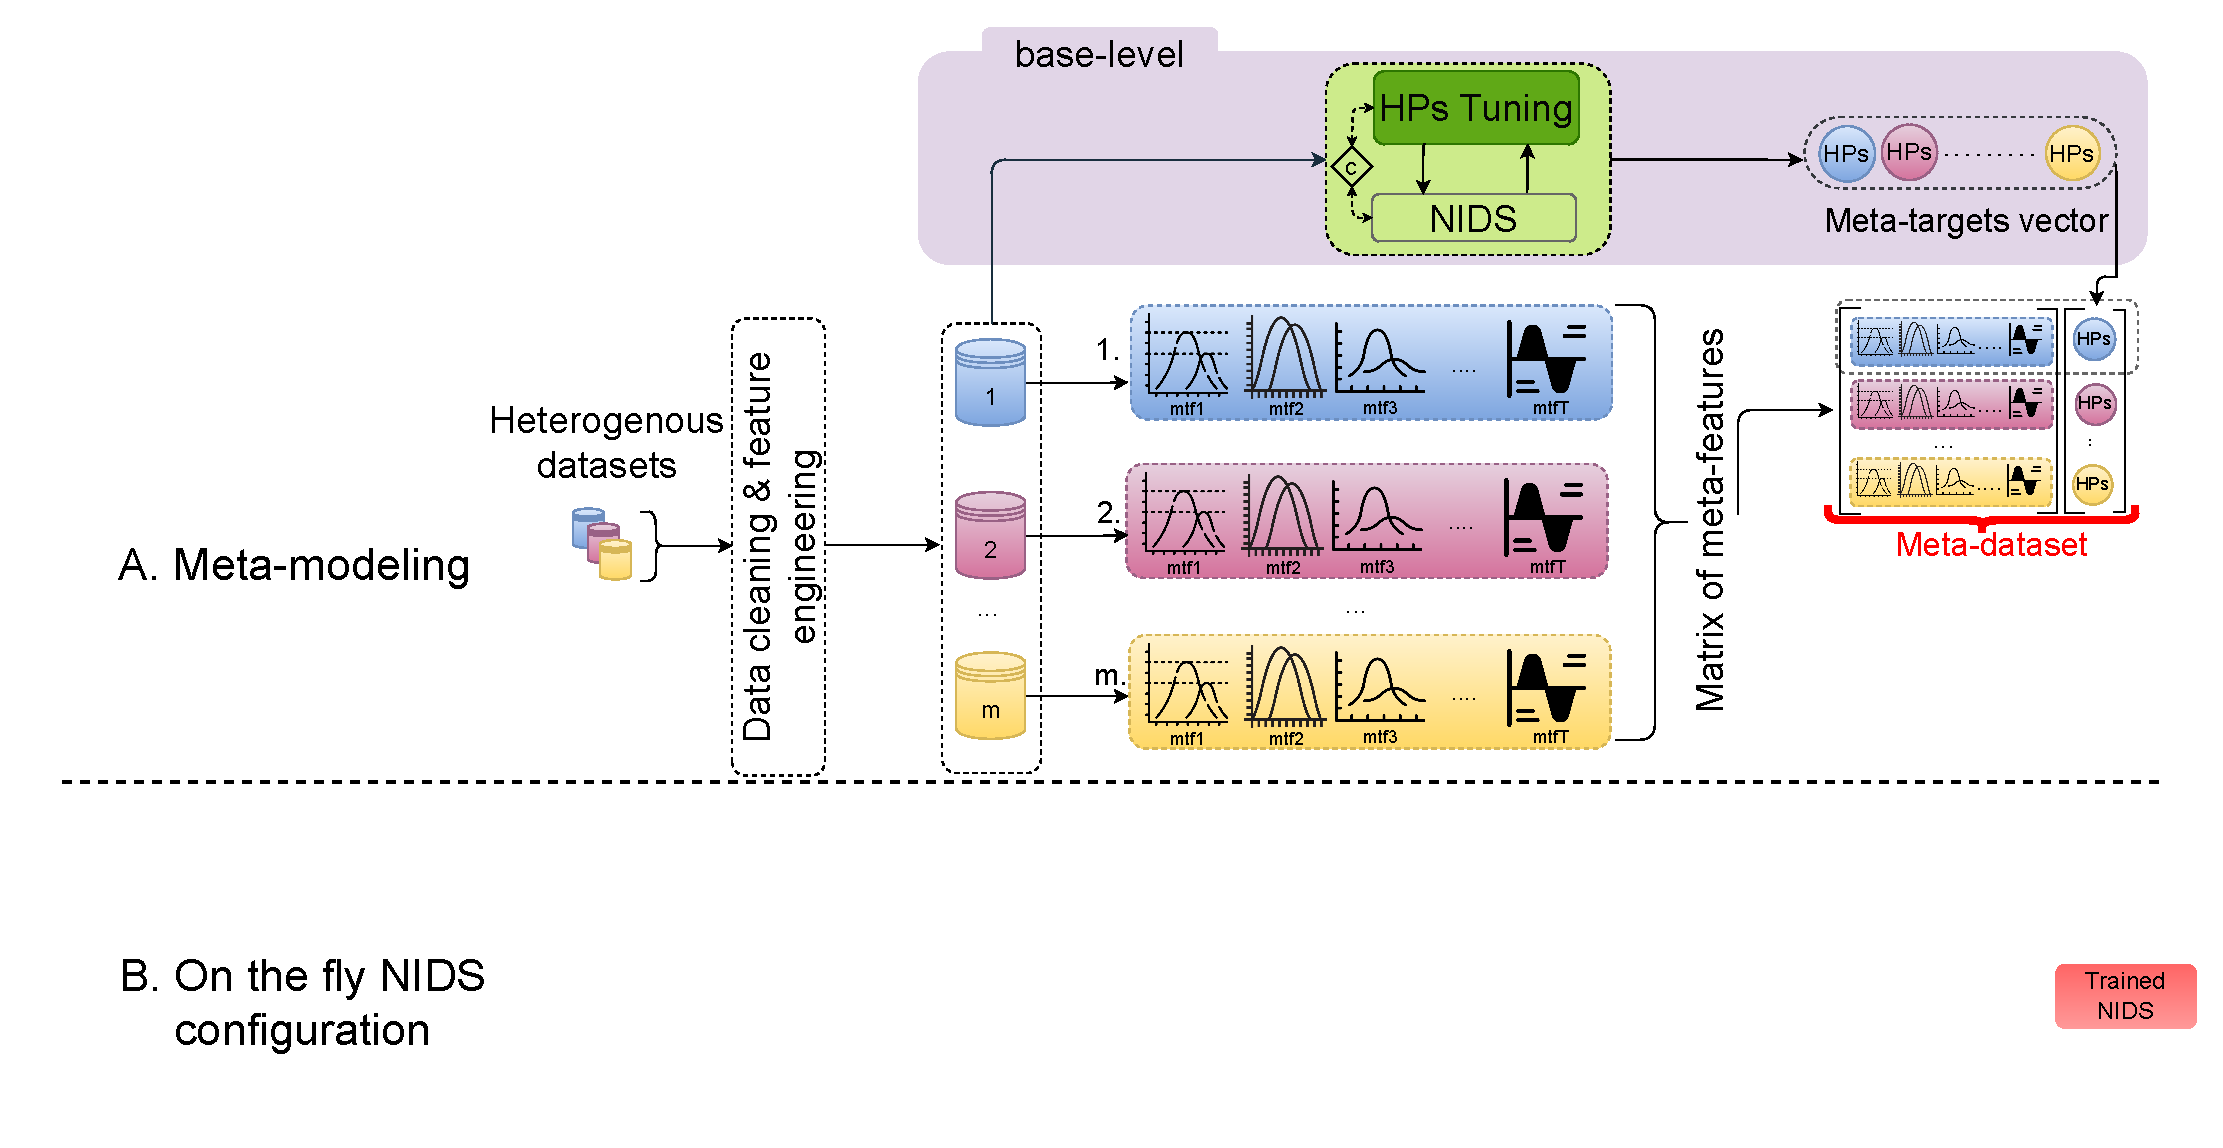
\includegraphics[width=\linewidth]{figures/auto_configuration/method/secondPartPage6.pdf}
\end{frame}

\begin{frame}[noframenumbering]{Auto-configuration via Meta-learning}
	\centering
	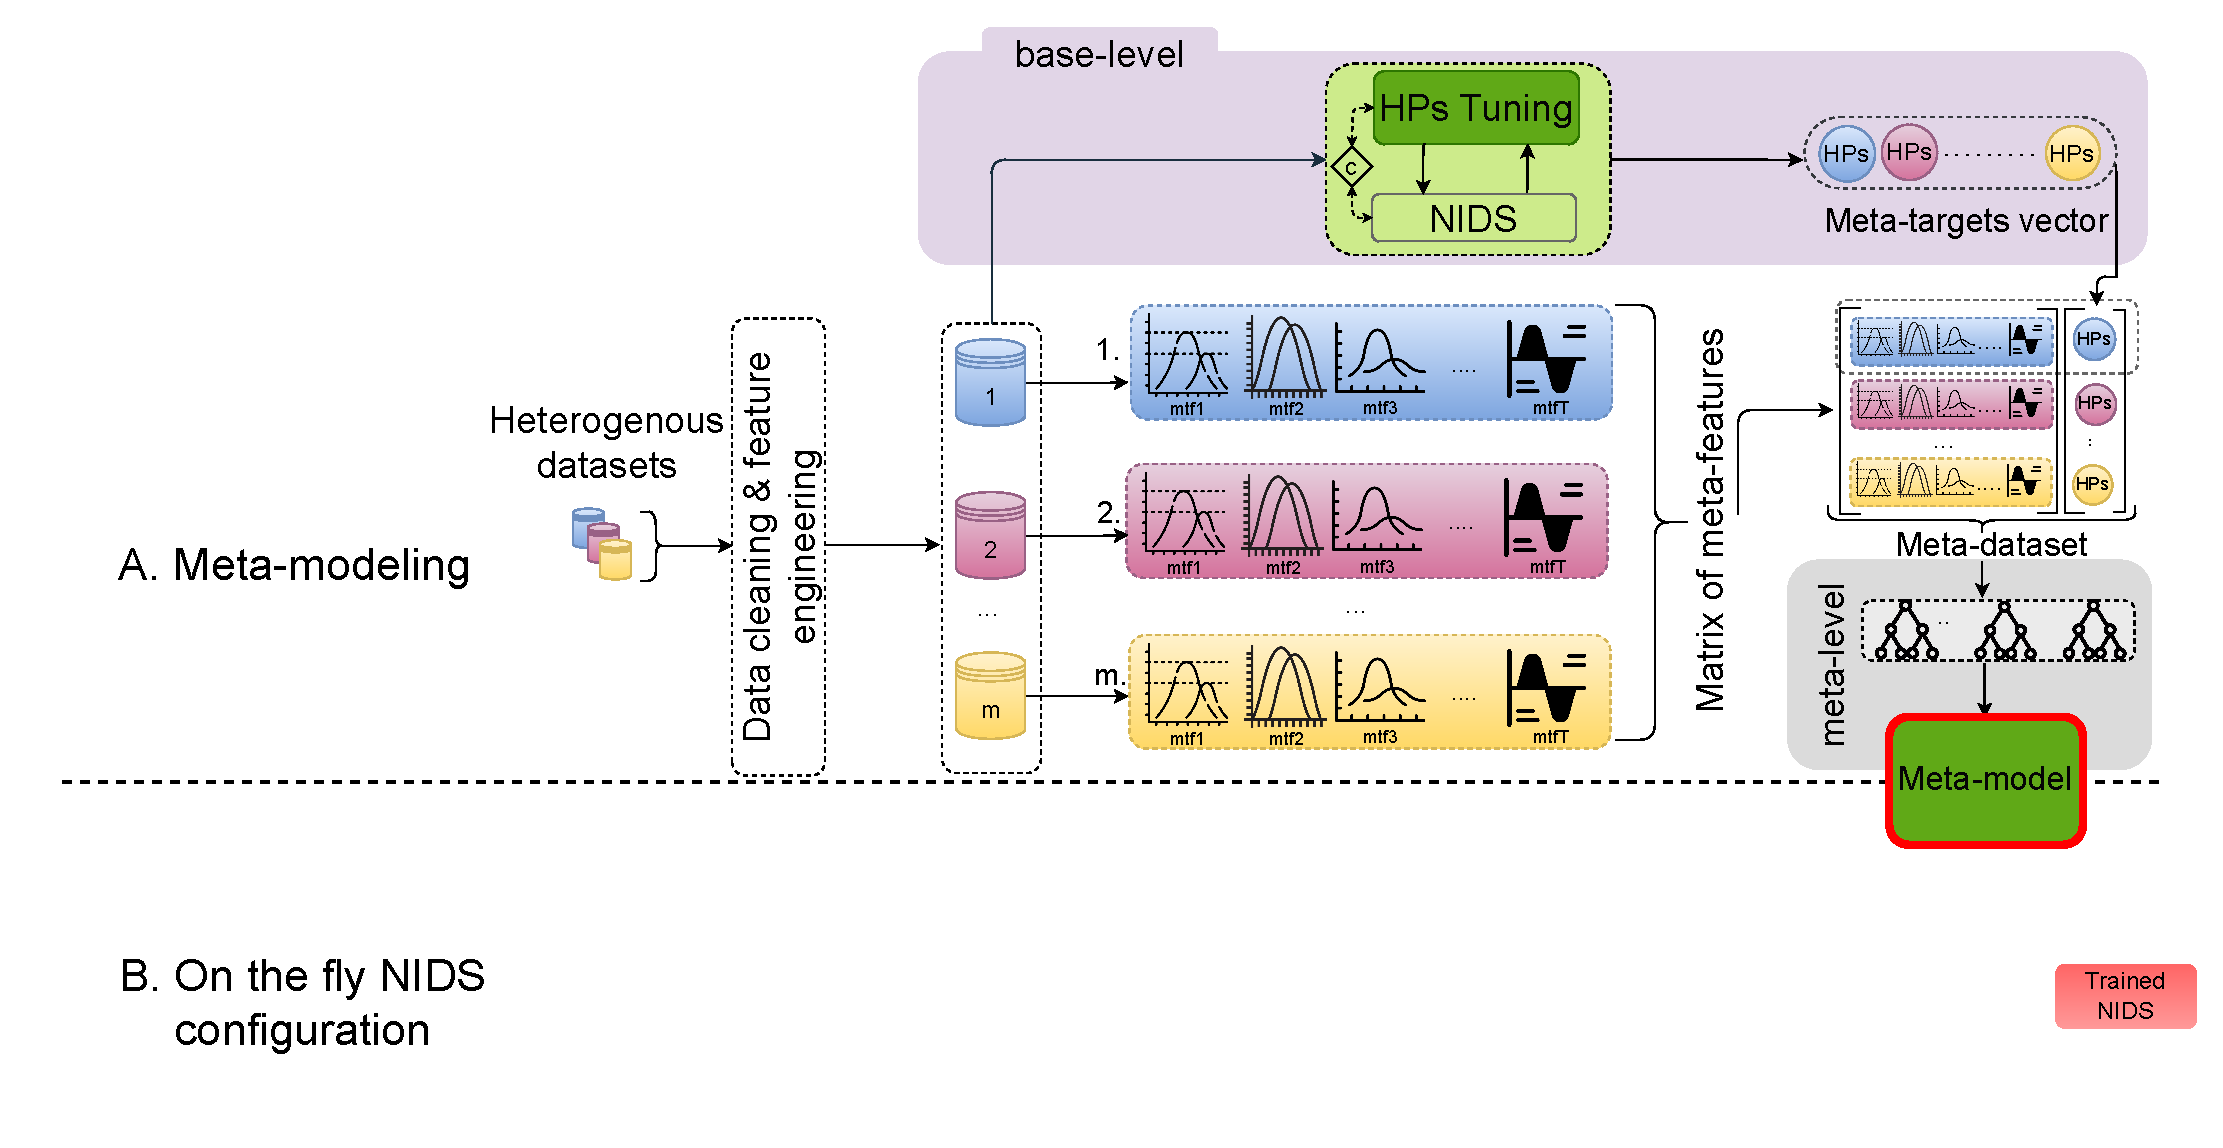
\includegraphics[width=\linewidth]{figures/auto_configuration/method/secondPartPage7.pdf}
\end{frame}

\begin{frame}[noframenumbering]{Auto-configuration via Meta-learning}
	\centering
	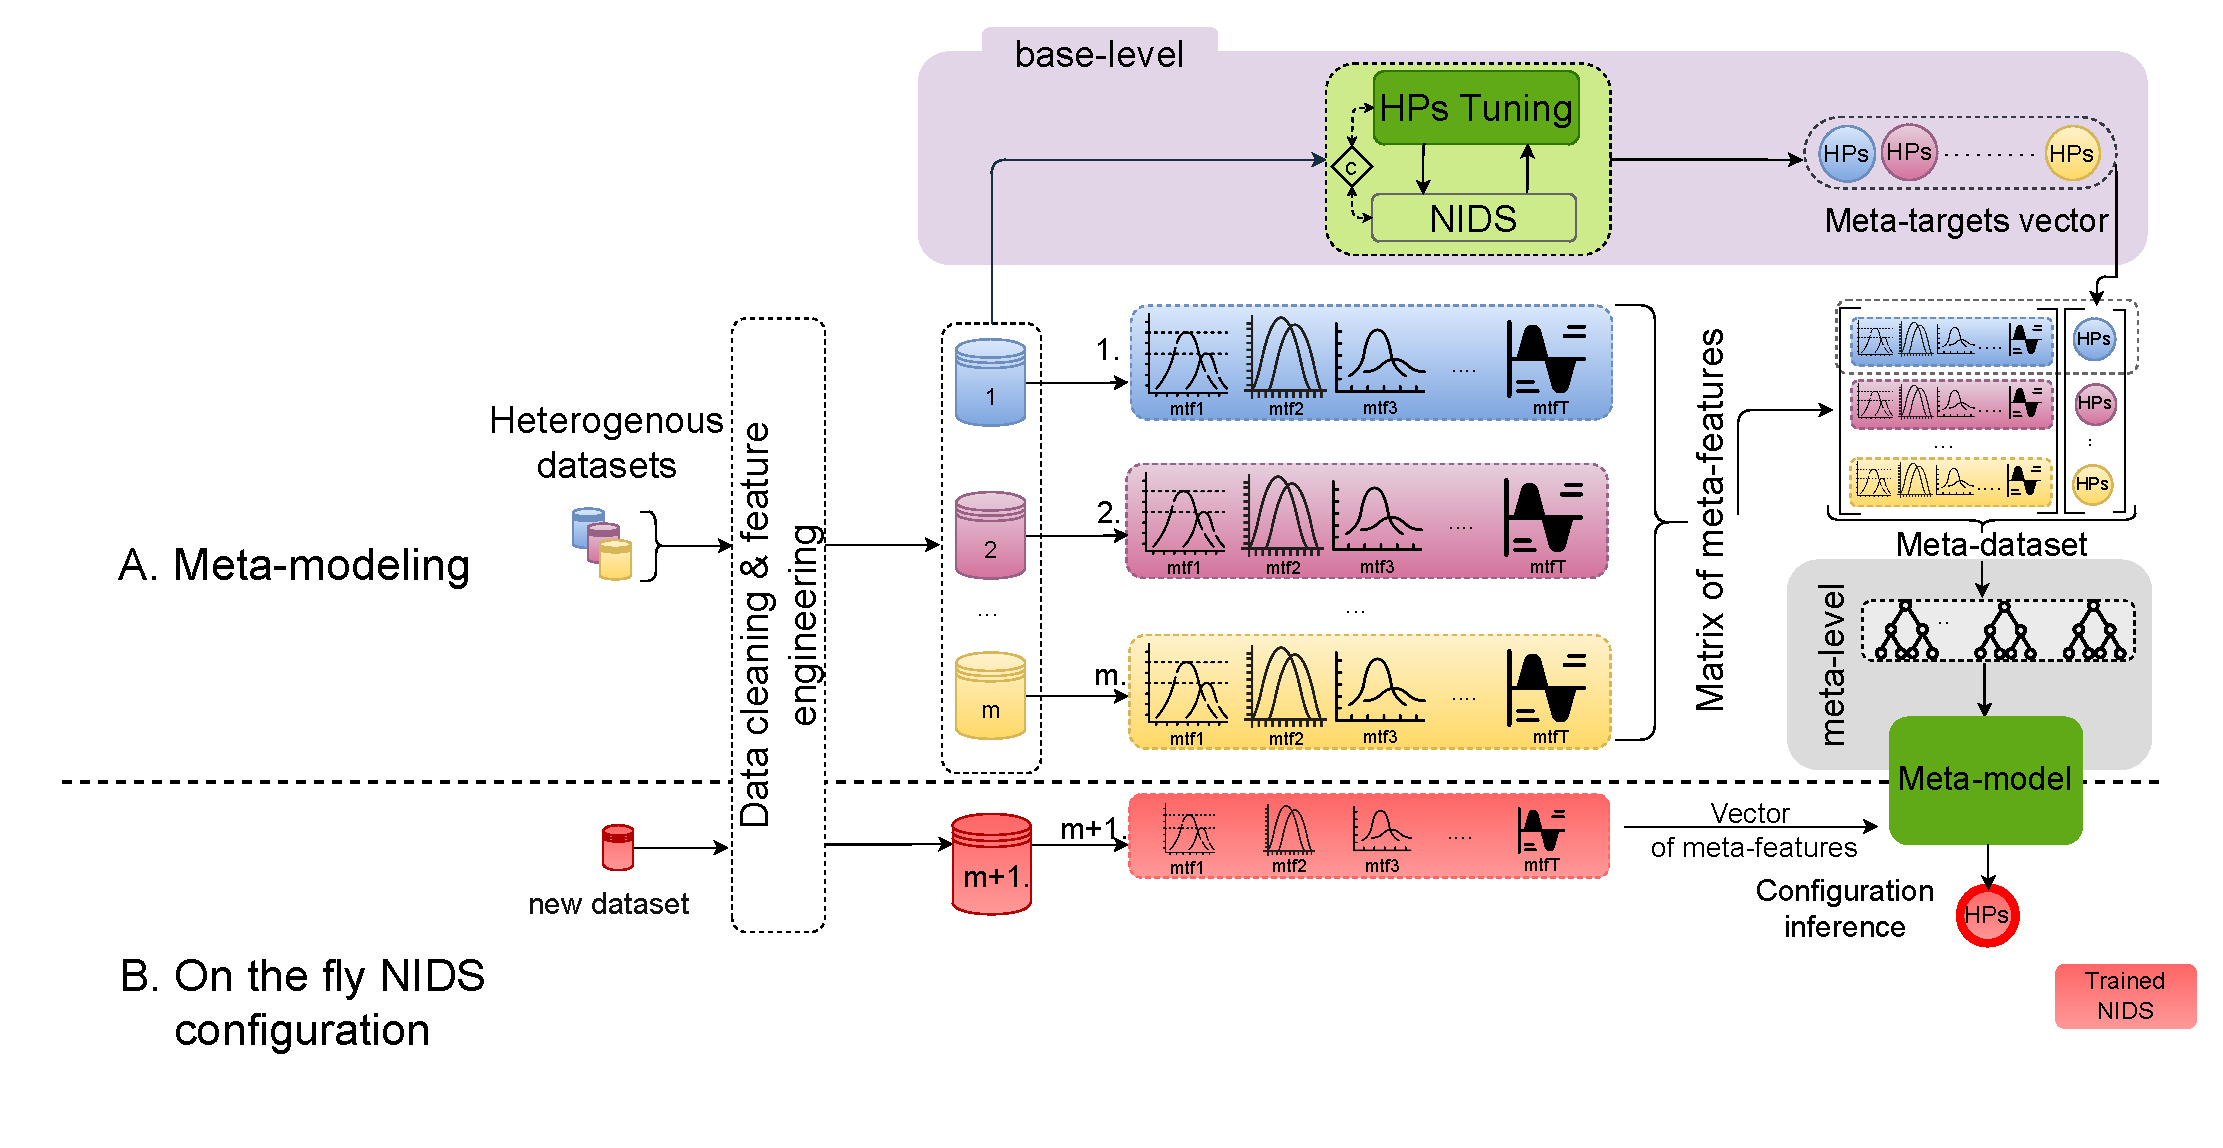
\includegraphics[width=\linewidth]{figures/auto_configuration/method/secondPartPage8.pdf}
\end{frame}

\begin{frame}[noframenumbering]{Auto-configuration via Meta-learning}
	\centering
	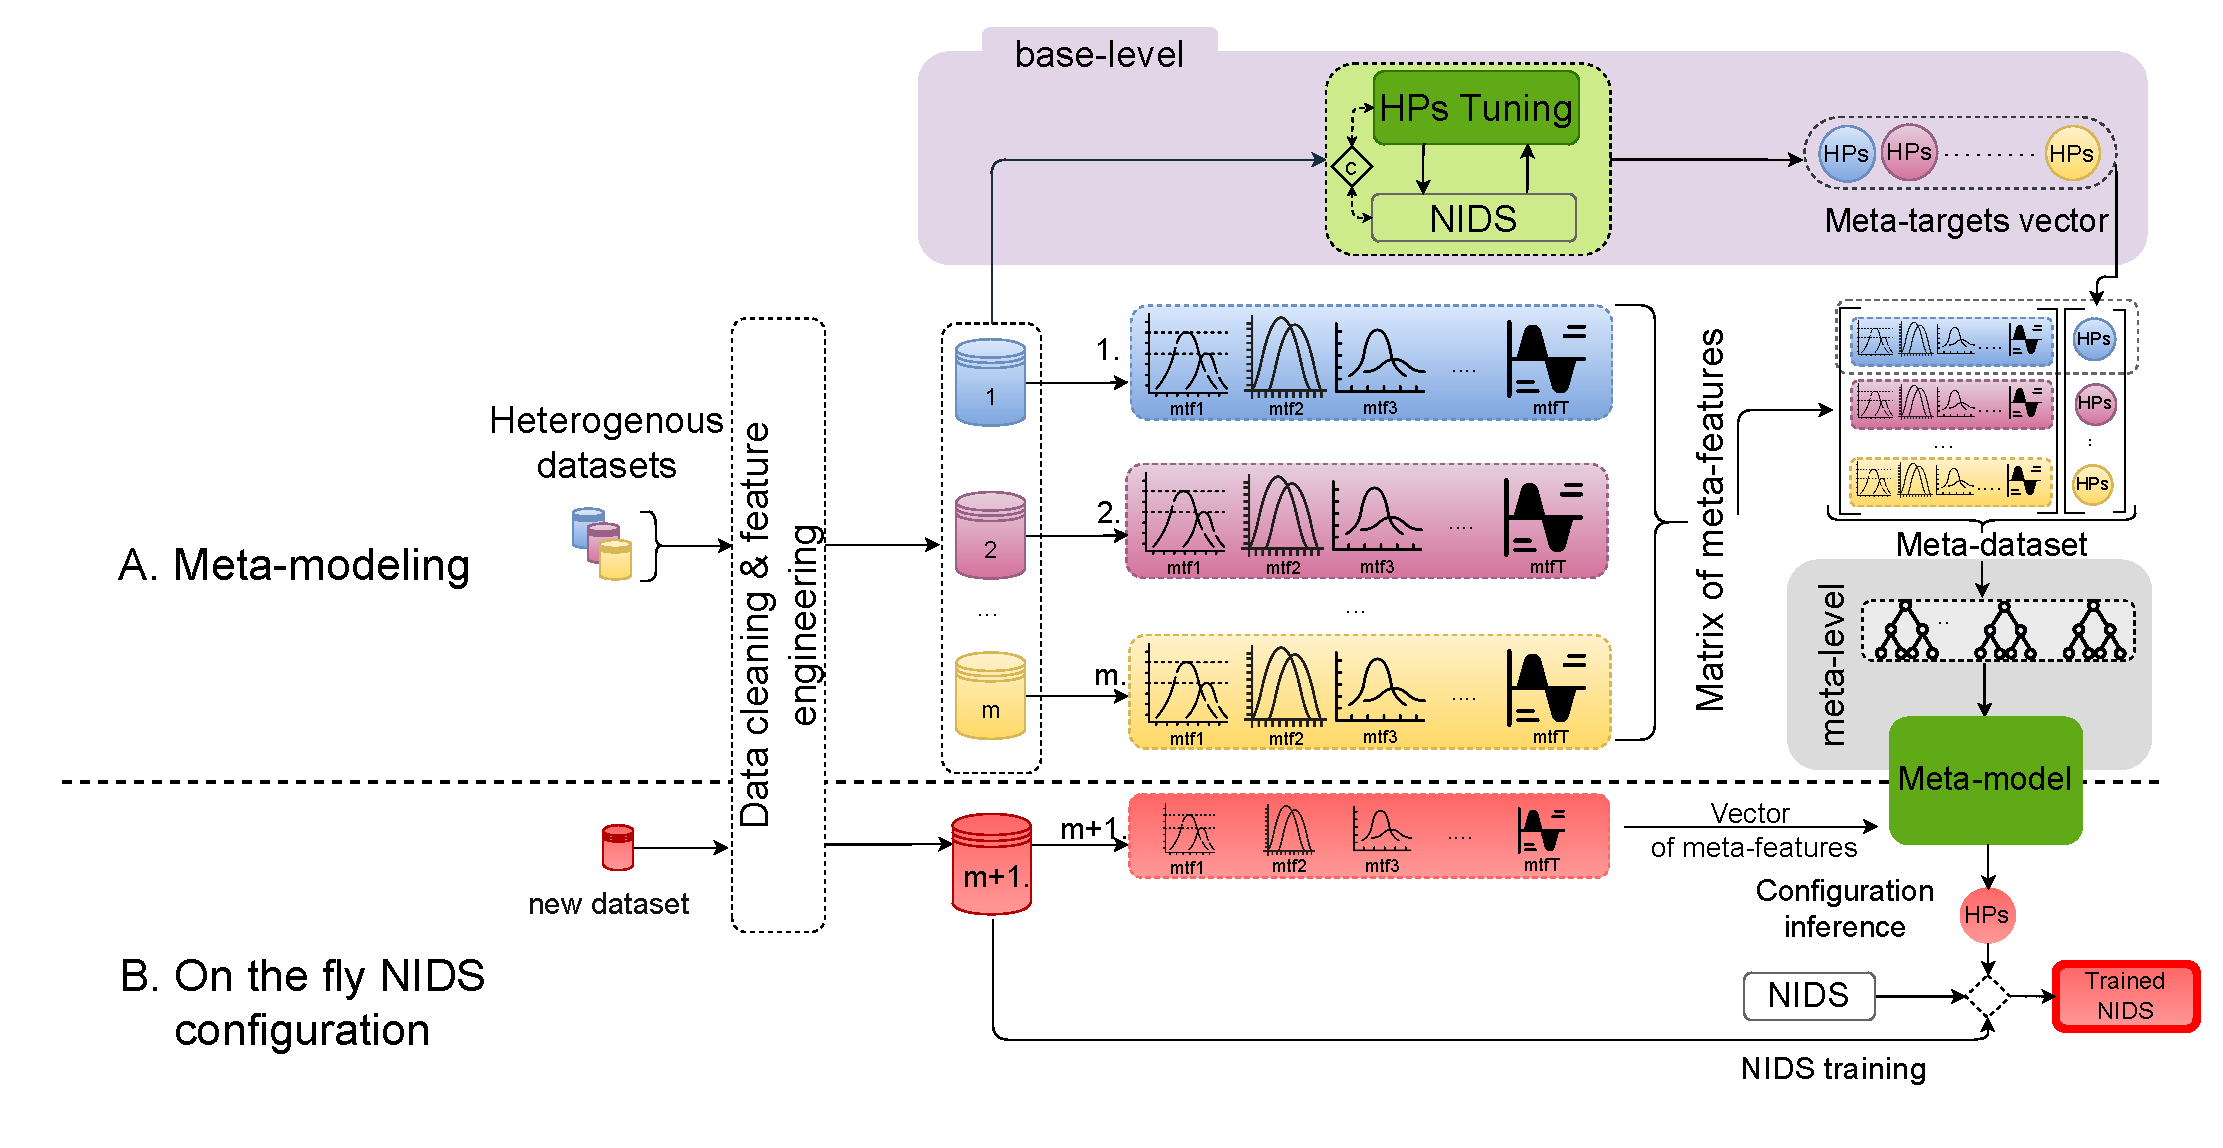
\includegraphics[width=\linewidth]{figures/auto_configuration/method/secondPartPage9.pdf}
\end{frame}
